\chapter{Indledning}
Hensigten med dette projekt, er at udvikle spillet "Goofy Candygun 3000". Spillet går ud på at 1-2 spillere dyster om, at ramme et mål med slik, affyret fra en slikkanon, styret af en Wii-Nunchuck controller. For at finde inspiration til projektet, og idéer til implementering, blev der søgt efter lignende projekter på internettet. Det viste sig, at idéen med at skyde med slik, ikke er en original idé, da lignende projekter såsom "The Candy Canon" \cite{Website:CandyCanon} allerede findes. Til forskel fra The Candy Cannon og lignende projekter som affyrer projektiler uden et egentlig formål, vil der i dette projekt blive udviklet en kanon til brug i et spil. Kanonen affyres og styres af spillerne via en controller. Altså skal projektet ende med en kanon som indgår i et to personersspil, f.eks. til brug ved fester og andre sociale begivenheder.
Målet med projektet, er at bygge en funktionelt prototype, samt at dokumentere dette med en projektrapport og dens dertilhørende dokumentation. 
Det følgende afsnit beskriver, hvilke krav der stilles til projektet fra IHA's side.

\section{Krav til produktet}
Dette projekt tager udgangspunkt i projektoplægget for 3. Semester projektet, præsenteret af \textit{Ingeniørhøjskolen, Aarhus Universitet}. Til dette projekt er der ikke stillet krav til typen af produkt der skal udvikles, dog er der sat krav til hvad produket skal indeholde. Disse krav er som følge:

\begin{itemize}
	\item{Systemet \textit{skal} via sensorer/aktuatorer interagere med omverdenen}
	\item{Systemet \textit{skal} have en brugergrænseflade}
	\item{Systemet \textit{skal} indeholde faglige elementer fra semesterets andre fag}
	\item{Systemet \textit{skal} anvende en indlejret Linux platform og en PSoC platform}
\end{itemize}

På baggrund af disse krav er der udarbejdet et produkt, der beskrives i afsnit \ref{afsnit:systembeskrivelse}.

I dette projekt bliver produktet opbygget som en prototype. Grundet dette er der i afsnit \ref{afsnit:analyse} beskrevet nogle grundlæggende hardwarekomponenter til realisering af denne prototype.

\section{Systembeskrivelse}
\label{afsnit:systembeskrivelse}
I dette projekt skal der udvikles en slik kanon til spillet \textit{Goofy Candygun 3000}. Denne slik kanon skal kunne skyde med slik, eksempelvis M\&M’s eller Skittles. Kanonen der afyrer slikket, skal styres af spillerne via en Wii-Nunchuck controller. 

Et typisk brugerscenarie er, at spillerne bestemmer antallet af skud for runden. Når dette er gjort, er spillet igang. Herefter går Wii-nunchucken på skift mellem spillerne for hvert skud. Dette fortsættes indtil skuddene er opbrugt. Vinderen er spilleren med flest point. Spillets statistikker vises løbende på brugergrænsefladen. Dette brugerscenarie er illustreret i det rige billede på figur \ref{fig:RigtBillede}.

\begin{figure}[H]
	\centering
	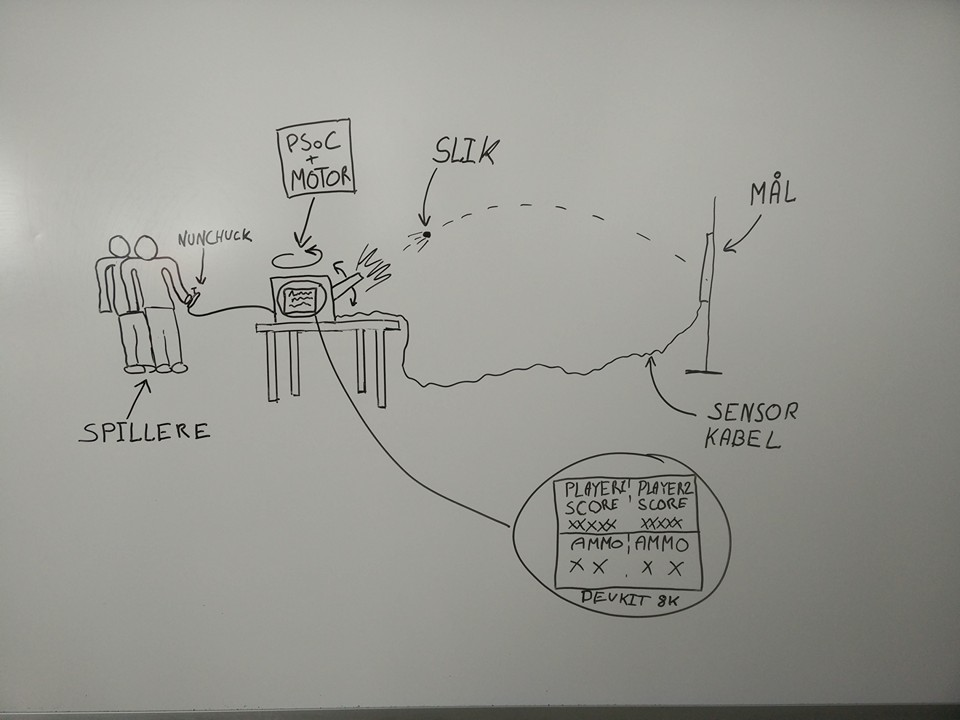
\includegraphics[width=\textwidth]{Projektformulering/images/rigtBillede}
	\caption{Rigt Billede af det endelige produkt}
	\label{fig:RigtBillede}
\end{figure}

Det endelige produkt omfatter:
\begin{itemize}
	\item{En brugergrænseflade, hvor brugeren kan initiere både system test og selve spillet. Derudover kan brugergrænsefladen vise:}
	\subitem{Point}
	\subitem{Kanonens vinkel}
	\subitem{Antal resterende skud}
	\item{En eller flere motorer, der drejer kanonen om forskellige akser}
	\subitem{Disse skal styres med en Wii-nunchuck controller}
	\item{Et mål, der kan registrere spillernes skud}
\end{itemize}


\section{Rigt Billede}

På figur \ref{ref:RigtBillede} ses et rigt billede af det ønskede produkt. Billedet beskriver brugerscenariet.

\begin{figure}[H]
	\centering
	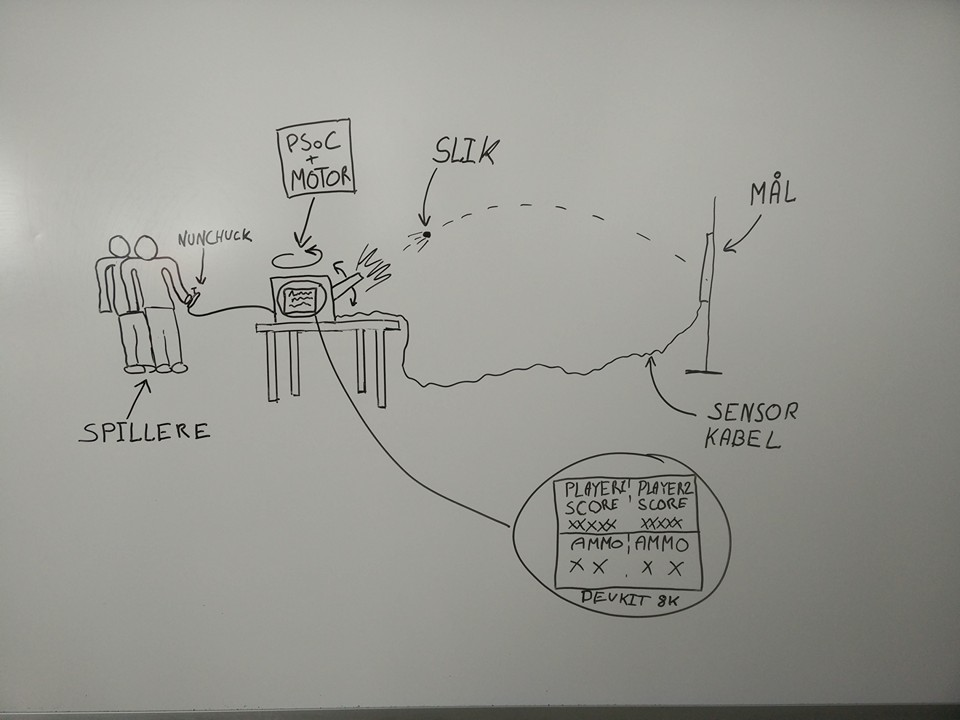
\includegraphics[width=\textwidth]{Projektformulering/images/rigtBillede}
	\caption{Rigt Billede af det endelige produkt}
	\label{ref:RigtBillede}
\end{figure}


%\section{Ansvarsområder}
%I løbet af projektet vil projektgruppen blive opdelt i to hovedgrupper - 'hardware' og 'software'. Softwaregruppen vil desuden stå for grænsefladeprogrammering mellem software og hardware. Disse grupper vil have til ansvar at designe og implementere hhv. hardware og software til projektet. Hardwaregruppen vil bestå af de personer, der læser til elektroingeniør (Mikkel Nielsen og Pernille Kjeldgaard). Softwaregruppen vil bestå af de personer, der læser til IKT-ingeniør (Kasper Rieder, Michael Kloock, Tenna Rasmussen, Mia Konstmann og Daniel Jensen).
